\documentclass[tikz]{standalone}
\usepackage{bm}
\usepackage{stix}

\tikzstyle{lin}=[rounded corners, fill=blue!30!white]
\tikzstyle{act}=[rounded corners, fill=orange!30!white]

\begin{document}
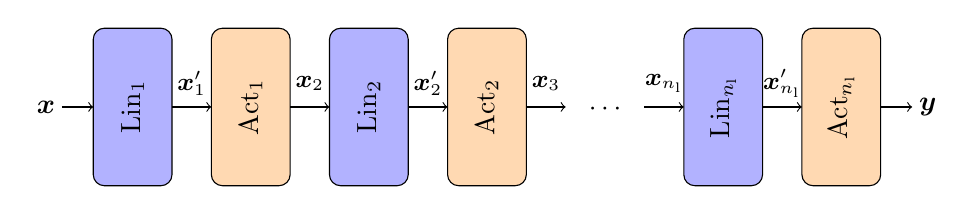
\begin{tikzpicture}

\draw[lin] (0  , 0) rectangle ++(1, 2);
\draw[act] (1.5, 0) rectangle ++(1, 2);
\draw[lin] (3  , 0) rectangle ++(1, 2);
\draw[act] (4.5, 0) rectangle ++(1, 2);
\draw[lin] (7.5, 0) rectangle ++(1, 2);
\draw[act] (9  , 0) rectangle ++(1, 2);

\node[rotate=90] at (0.5, 1) {Lin$_1$};
\node[rotate=90] at (2  , 1) {Act$_1$};
\node[rotate=90] at (3.5, 1) {Lin$_2$};
\node[rotate=90] at (5  , 1) {Act$_2$};
\node[rotate=90] at (8  , 1) {Lin$_{n_\mathrm{l}}$};
\node[rotate=90] at (9.5, 1) {Act$_{n_\mathrm{l}}$};

\draw[->] (-0.4, 1) -- ( 0  , 1);
\draw[->] ( 1  , 1) -- ( 1.5, 1);
\draw[->] ( 2.5, 1) -- ( 3  , 1);
\draw[->] ( 4  , 1) -- ( 4.5, 1);
\draw[->] ( 5.5, 1) -- ( 6  , 1);
\draw[->] ( 7  , 1) -- ( 7.5, 1);
\draw[->] ( 8.5, 1) -- ( 9  , 1);
\draw[->] (10  , 1) -- (10.4, 1);

\node at (-0.6, 1) {$\bm{x}$};
\node at (10.6, 1) {$\bm{y}$};
\node at (6.5, 0.97) {$\cdots$};

\node at (1.25, 1.3) {\small $\bm{x}'_1$};
\node at (2.75, 1.3) {\small $\bm{x}_2$};
\node at (4.25, 1.3) {\small $\bm{x}'_2$};
\node at (5.75, 1.3) {\small $\bm{x}_3$};
\node at (7.25, 1.3) {\small $\bm{x}_{n_\mathrm{l}}$};
\node at (8.75, 1.3) {\small $\bm{x}'_{n_\mathrm{l}}$};

\end{tikzpicture}
\end{document}
